\documentclass[a4paper]{article}
\usepackage{url}
\usepackage{graphicx}

\newcommand{\TODO}[1]{
\begingroup{\noindent\textbf{TODO:\ #1}\par\medskip}\endgroup%
}
\def\mmeta#1{\emph{$\cal MET\!\!A$#1$^2$}}
\long\def\FIXME#1{{\medskip\par\noindent\textbf{FIXME:} \sl #1\par\medskip}}

\title{Technical Report---Virtual Clusters as a New Service of MetaCentrum, the Czech NGI}
\author{Miroslav Ruda \and Zden\v ek \v Sustr \and Ji\v r\' i Sitera \and David Anto\v s \and Luk\'a\v s Hejtm\' anek \and Petr Holub \and Milo\v s Mula\v c}
%\author{Ruda, M.;
%\v Sustr, Z.;
%Sitera, J.;
%Anto\v s, D.;
%Hejtm\' anek, L.;
%Holub, P.;
%Mula\v c, M.}
%\institute{CESNET, z. s. p. o., Zikova 4, 160~00 Prague, Czech Republic}

\hyphenation{PBSPro Meta-Centrum Booot Pe-run}

\widowpenalty=10000
\clubpenalty=10000
\begin{document}
\maketitle


\begin{abstract}
MetaCentrum, the Czech NGI, started to virtualize the infrastructure several years ago.
The virtual nature of the resources, being integrated with the resource management system, is mostly hidden to end users.
We are introducing a new public service ``virtual cluster'' which turns the virtualized infrastructure
into end user service. Virtual cluster service provides an illusion of totally dedicated clusters
running on a shared infrastructure under complete user control, including administrator access and
user specified application environment. Virtual machines and clusters are handled in a way similar to
ordinary computation jobs, planned for batch or interactive processing. We developed an extension to
job scheduler PBSPro and new management tools to smoothly integrate virtual cluster service into
production environment. Networking is a vital part of the service, where Czech NREN CESNET2
technology allows managing virtual cluster network without perceivable overhead. Virtual network
is seen as a new resource.

This report is an extended version of the paper
called ``Virtual Clusters as a New Service of MetaCentrum, the Czech NGI,'' which was presented
at CGW~2009.

\noindent{\bf Keywords:} virtualization, batch system, cloud, virtual appliance
\end{abstract}

%Pridano pro jednodussi orientaci ve strukture a jejich zmenach, mozno nasledne zase zlikvidovat.
%\tableofcontents

\section{Introduction}

In recent years, virtualization of computing resources became one of key focal points of research and development
in MetaCentrum (\url{http://meta.cesnet.cz}). It allows applications with contradictory environment requirements to run on a single node, making it rather simple
to allocate resources available to each of them.

This year, MetaCentrum
introduces another step in development relying on the principles of virtualization---\emph{virtual clusters} enhanced with features
inspired by cloud computing, but oriented primarily on HPC user communities. The new solution allows users to request specific environment for their applications,
or even supply their own virtual images (appliances) to replace defaults made available by the service provider. Such images may be used to set up temporary
virtual clusters with a requested number of nodes, or to temporarily extend existing physical clusters with additional virtual nodes to handle peak loads.

The possibility to use custom images tuned to the needs of a specific application while setting up virtual clusters lowers the adoption threshold for potential new
users since the resulting virtual environment does not differ in any significant way from their current traditional environment.

\section{Architecture Overview}
\label{Architecture}

\begin{figure}[htb]
\begin{center}
    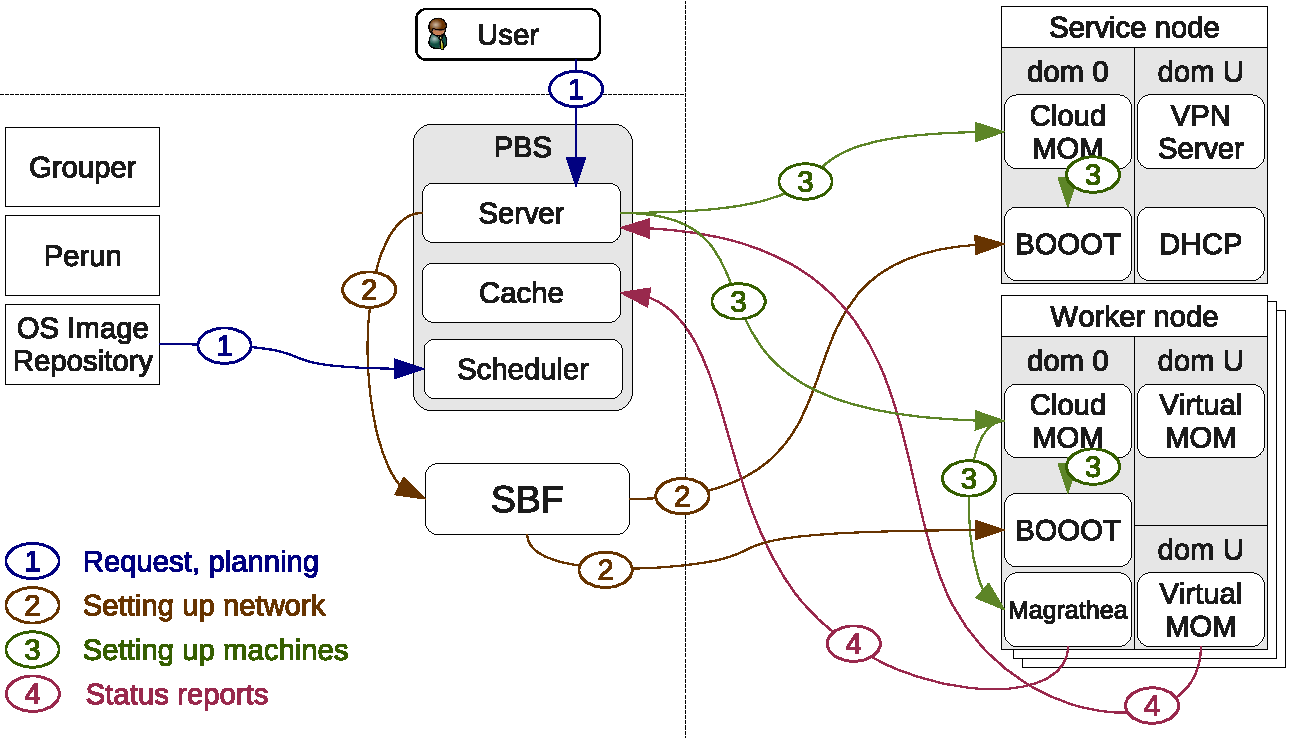
\includegraphics[width=.8\columnwidth]{cloud_arch.pdf}
\end{center}
    \caption{Overall architecture of the virtual clouds solution}
    \label{fig:architecture}
\end{figure}

Several services (Fig.~\ref{fig:architecture}) had to be combined and adjusted to implement the functionality. Scheduling is done by MetaCentrum's PBSPro batch system, virtual image
handling and management is being carried out by Magrathea, virtual clusters are managed with SBF and virtual LANs interconnecting individual cluster nodes
rely on the advanced capabilities of the CESNET2 NREN.

PBS is the core service. It had to be modified to support new types of jobs (virtual clusters) and to communicate with Magrathea and SBF, requesting virtual machines and private networks as per user requirements. More extensions were required to implement authorization, allowing cluster owners to specify authorized users of their clusters by referencing system-wide groups.

With its new capabilities, PBS Server accepts requests for virtual
clusters. PBS Scheduler then selects suitable machines, considering those
in \emph{down-bootable} state or those already running the requested image.
In the latter case, obviously, the resource must be free and still may not
be considered if the request does call for a private network to be
established. Machine status information is provided to the Scheduler by
Magrathea, with information mapping virtual nodes to physical machines
being available in PBS Cache. Virtual machine requests are then forwarded
to processes running in the hosting domain. A prologue within a container job runs Magrathea and Booot to install and start up the appropriate virtual image.

Similar to virtual cluster creation, cluster termination is also controlled
by the PBS Server, initiated either by the user or by elapsing an allotted timeslot. The Server uses Magrathea and Booot to stop and clean up the virtual machines, remove records from PBS Cache, and deactivate the private network where applicable.

Magrathea \cite{sc07} is an in-house developed system serving as an interface between the batch scheduling system and virtual machine monitors. It carries out
functions such as setting up, booting or terminating virtual machines, and provides essential feedback on the status or availability of physical
resources.

Booot is a service used for virtual domain management, i.e., installation, update and uninstallation of virtual domains. The domains are installed from image repository and configured by a set of enclosed scripts.

SBF is a tool used by the extended PBS to set up virtual networks~\cite{sbf}. Once a virtual cluster job is scheduled and physical resources selected, SBF may be called by the PBS Server to establish a private network. The ability to insert custom virtual clusters into their separate virtual networks is vital from the security viewpoint. By allowing custom images, the service
provider (MetaCentrum) relinquishes control of security within the cluster but encapsulates it in a private network to provide protection in both directions (protecting the
machines inside to allow the use of unpatched or outdated systems as required by users, while simultaneously protecting the outside world in case the virtual
cluster gets compromised), making the network accessible through a gateway and defining external resources accessible to machines within the network.

\section{Magrathea---Scheduling Virtual Machines}
\label{magrathea}

The Magrathea System~\cite{sc07} has been developed to provide management of several virtual
machines running on a single computer and submit jobs to the proper ones.

Magrathea provides an interface between the batch scheduling system and virtual
machine monitors. It allows jobs to be submitted in a controlled manner into virtual
machines running on cluster nodes (with multiple virtual machines running on a single
cluster node). Magrathea can also be seen as a scheduler running on each cluster node,
scheduling virtual machines according to jobs submitted by batch scheduling systems.
Instead of simplest approach via replacing each ``computational job'' with
``virtual machine running simple job'' we have chosen more general implementation, 
providing full layer for management of virtual machines on physical nodes, 
with ability to run several jobs in the same virtual machine sequentially or in parallel, 
but also with functionality where each job can be run in
virtual machine setup according job specific needs.

Furthermore, Magrathea is designed to be independent on
a batch system and virtual machine monitors used on computational
nodes---current implementation supports  the PBSPro batch system (and port to Torque system is in the 
current roadmap) and Xen and VServer virtual machine monitors (with generic interface, which should 
be sufficient to implement support for other virtualization techniques like KVM or LXC).

\subsection{Original Use Cases}
Development of Magrathea has been originally driven by several use cases:

\begin{description}
\item[Multiple static domains,] only one of them may run at any given time, using 
exclusively the physical resource.
Typically used for sharing nodes between mutually
incompatible projects. A single domain, running actual computational job, is assigned almost 
all available resources at a time, while the other domains are allowed to run with 
a minimum CPU and memory consumption,
just to appear available to their respective scheduling systems.

\item[High-priority jobs in privileged domains,]
such as interactive jobs required to run immediately, or massively parallel 
jobs whose processing would
be unfeasible should they have to wait until the full number of required processors is
actually free, may run in high-priority or ``privileged'' domains,
temporarily suppressing resources available to standard virtual domains. Jobs
in the standard domains are suspended, but still visible to
their respective scheduling and monitoring systems. This ensures that those
suspended jobs are not considered ``lost'' or aborted, and the
scheduler does not resubmit them to another node. The same technique of domain preemption
is used for giving cluster owners higher priority, while providing resources to rest 
of grid when cluster is not used.
\item [Suspending/freezing virtual machines] in order to run
services that only need to be available temporarily. Such machine or service can be 
suspended on demand, remain on ``stand-by'' and get reactivated quickly by service owner
when needed, instead of slow booting of all the nodes.
\end{description}

\subsection{Virtual Cluster Motivations}
Virtual clusters consist of virtual machines rather than actual physical ones,
abstracting from the physical topology of the underlying resources. This service
resembles, to certain extent, motivation for clouds ---virtual computing services
whose popularity has been growing in recent years.

Two additional use cases have been kept in mind while implementing functionality
required by virtual clusters:

\begin{description}

\item[Jobs running in an environment adjusted to their needs.] 
Jobs may require specific environment to run, installed for each job run separately 
from registered node images (appliances). Users may be allowed to
supply their own images, tuned specifically for compatibility with their applications.

\item[Virtual nodes used to form semi-permanent
virtual clusters] that may be only used for running specific
jobs, and consequently removed or kept back for future need. Jobs in such virtual
clusters may be managed either by central PBSPro installation provided by MetaCentrum
or may become an integral part of user's infrastructure,
subject to a common job and account management. With the latter approach, existing 
physical resources (clusters) may be
extended with additional virtual nodes, and physical or virtual nature of any given
node is completely transparent to the user.
\end{description}

\subsection{Architecture Extensions}

Several extensions to Magrathea implementation (for a full description of the architecture see~\cite{sc07})
were needed---support for user-supplied images and support for nodes where system is to be installed on the fly.

\subsubsection{User-supplied Images}
In its original design, Magrathea process had to be installed inside each virtual machine, to allow 
easier management of booting and suspend/resume operations. Current implementation supports a special type 
of node images, where this modification of user-supplied image is no longer required. In such case, image 
specification contains also estimation of booting time, after which the
node is treated as booted and the Magrathea system 
is not waiting for a confirmation message from process installed inside of
a virtual machine.

\subsubsection{Magrathea Status}
\begin{figure}[ht]
\begin{center}
    
\includegraphics[width=\columnwidth]{frozen}
    \caption{States and transitions between them for frozen
        virtual machines.}
    \label{fig:frozen}
\end{center}
\end{figure}

Largest changes to the Magrathea system were required to support dynamic node installation, using an image specified in 
job description.  Magrathea status of a virtual machine (used by the scheduling system, see Section \ref{pbs}) represents
state of the virtual machine for other scheduling systems like PBSPro.
Original states, depicted on 
Figure~\ref{fig:frozen},
represent various states of running virtual machines. A virtual machine is \textit{free} (available for new jobs), when 
there are resources available for this domain (no other domain is already running jobs). 
If a domain in running jobs (is in state \textit{running}), 
remaining domains are in \textit{occupied} state, representing situation,
when node is considered free in PBS monitoring, but 
virtual machine cannot get resources in Magrathea. The Magrathea system
represents also preemptible domains, when a domain 
in \textit{running-preemptible} state can be preempted by privileged domain (standard domains becomes \textit{preempted}, 
while high-priority domains becomes \textit{running}). Similarly, a privileged domain can be \textit{frozen}
and later resumed, while a standard domain is \textit{running} and \textit{preempted} respectively.

For virtual cluster support, Magrathea status was extended 
to represent not only existing and running nodes, but also nodes which are not running, but may be potentially 
installed and booted. Current version of Magrathea supports complete management of VM life-cycle, including 
node preparation, boot and shutdown, see Figure~\ref{fig:lifecycle}.

\begin{figure}[htb]
\begin{center}
    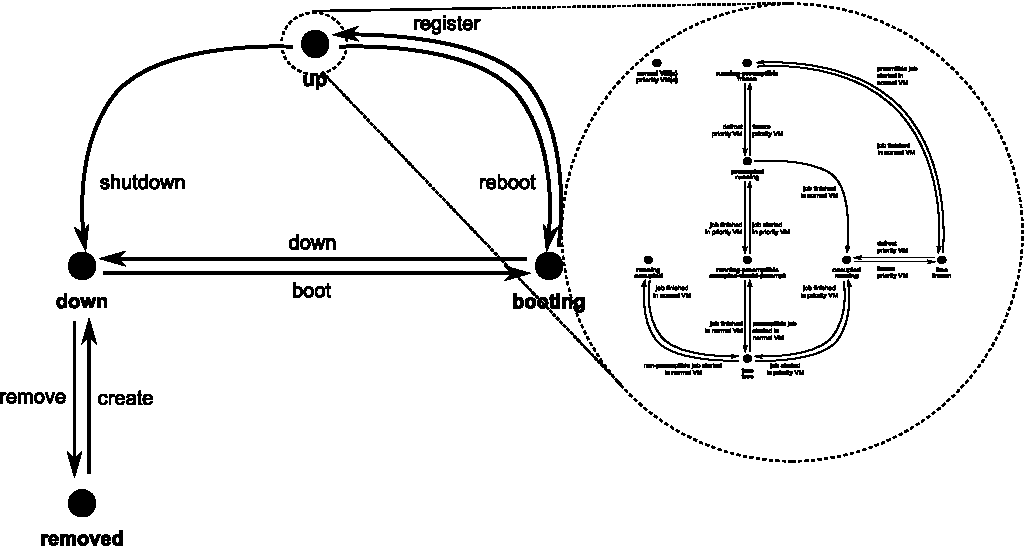
\includegraphics[width=\columnwidth]{lifecycle2}
    \caption{States and transitions between them for bootable nodes}
    \label{fig:lifecycle}
\end{center}
\end{figure}

New state \textit{down} represents a virtual node which is not running and cannot be booted automatically, state
\textit{down-bootable} represents a virtual node which can be booted on request. During booting
process, state of the node is \textit{booting}, while state of other domains running on the same physical node is 
changed to \textit{occupied-booting}.

\subsubsection{Preemption of a Running Domain}

Preemption overhead (time needed for domain preemption, especially for reducing memory of preempted domain)
is critical for the usability of preemption technique, especially for Xen implementation.
While standard Xen method called ballooning was sufficient for simple jobs, it is slow 
for intensive computations.  We have developed kernel helper module, utilizing suspend-to-disk 
functions from standard Linux kernel for more aggressive freeing memory which is than returned to Xen.
Implementation was verified on standard computational nodes in MetaCentrum
(2${}\times{}$dual-core nodes)
and also on nodes with larger memory and number of CPUs. In
Tab.~\ref{tab:pre}, we present results
from test scenario with 14 parallel CPU and memory intensive processes consuming 15GB of
memory, preemption swaps out 14.7GB and processes are stopped using SIGSTOP before
reducing the memory.

\begin{table}[h]
\begin{center} 
\begin{tabular}{|@{\ }r@{\quad}|@{\quad}r@{\ }l@{\ }|}
\hline
Disk speed & 2m & 50s\\
\hline
Magrathea implementation& 3m & 40s \\
\hline
Xen balloon driver & 41m & 20s \\
\hline
%w/o SIGSTOP & hours & \\
\end{tabular}
\label{tab:pre}
\caption{Time of preemption}
\end{center}
\end{table}

\subsection{Management of Virtual Images}

Management and deployment of virtual images is handled by a Magrathea
module called Booot. Booot scripts run on hypervisors (Dom0) of the
machines and a repository server.
The Booot repository server is an
implementation of an \textit{image repository}, which contains \textit{virtual appliances}~\cite{appliances}
(in the form of bootable images) together with metadata defining each appliance. The metadata contain
a description of the image is several following categories:
\begin{description}
\item[image maintenance:] image origin, owner, users allowed to use this image
\item[image requirements:] hardware architecture, number of CPU, necessary disk space
\item[image properties:]  properties of the installed OS; used in standard batch systems for selection
 of needed functionality (OS flavor)
\end{description}
The metadata is used by the PBS Scheduler for matching images and physical
nodes where to run them, for authorization decisions, and by deployment 
tools during the deployment phase.

\emph{Image deployment} tools support actual deployment of an image as well as configuration of the system within (network setup,
security keys assigned to this virtual image). Network setup is either static (predefined IPs and hostnames for virtual machines 
running ``certified'' images) or dynamic using DHCP.
The deployment tools reside
on hypervisors of computation host machines. 

\subsubsection{Domain Management}

Booot handles deployment of images and configuring new domains as well as
domain removal and data backup. Domains are created with the following command:

\begin{verbatim}
booot create [--dont-create-fs --no-image-copy|--think-about-copy|
             --copy-rsync|--copy-dd_balloon} [-help] DOMAIN_NAME

  --dont-create-fs    don't create FS on LV
  --no-image-copy     don't copy image
  --think-about-copy  use heuristics for choosing copy method
  --copy-rsync        use rsync method
  --copy-dd_balloon   use dd_balloon method
\end{verbatim}
and the deployment process goes as follows:

\begin{enumerate}
\item check whether all system utilities necessary for installation are
available in the hypervisor domain (e.g., rsync, dd, \dots)
\item gathering parameters needed for installation (command line
parameters, class parameters---see Section \ref{ic}, runtime
parameters---section \ref{rp})
\item check whether the domain is not (accidentally) running
\item creating logical volumes for installation (LVM)
\item creating filesystem on logical volumes
\item copying the image from repository
\item image configuration
\item uploading /scratch data
\end{enumerate}

\bigskip

Domain removal is done with command:
\begin{verbatim}
booot delete DOMAIN_NAME
\end{verbatim}
and uninstallation of domain proceeds in following steps:
\begin{enumerate}
\item check whether all system utilities necessary for installation are
available (e.g., rsync, dd, \dots)
\item gathering parameters needed for installation (analogical to
installation parameters)
\item check whether the domain is stopped (it has been stopped by
PBS and Magrathea)
\item backup of system logs
\item backup of /scratch
\item removal of the domain from the physical host
\end{enumerate}

\subsubsection{Image Repository}

Repository server stores images of virtual domains, their ssh keys and
keytabs, and scripts for domain customization. The data needed for
installation are downloaded from the repository server either via rsync or
using NFSv4 filesystem.

Downloads of sensitive data like krb5 keytabs or ssh keys are authorized by
host principal of Dom0 machine which initiates the download. We use remclt
to get keys and keytabs and rsh to manage/scratch files and logging data.

\subsubsection{Installation Classes}
\label{ic}

To customize installed domains, parameters like number of requested CPUs,
necessary disk partitioning, etc. need to be known and various
configuration files must be prepared. Booot introduces a concept of so
called \emph{installation classes}.

Domains running on similar hardware belong to one installation class and
share all configuration parameters and  customization scripts. A Booot
administrator then creates a mapping between domain name and installation
class it belongs to in a configuration file of Booot.

So, when Booot installs domain, it finds a class corresponding to installed domain and inherits all parameters and scripts defined for such class. Such scripts/parameters are therefore defined only once for a group of domains.

\subsubsection{Runtime Parameters}
\label{rp}

Customization scripts need also parameters which are not a~priori known
and are not available till PBS calls Booot (mainly IP address, domain
name). Such parameters are gathered by Booot and stored in one file to be
accessible for all scripts, either Booot scripts or customization ones.

\subsubsection{Customization Scripts}

Customization scripts are divided into two categories---Dom0 and DomU
scripts. Dom0 scripts are used to customize the installation in the
hypervisor domain, i.e., to customize the computation node ``from outside.''
They are controlled by the Booot administrator, without user access. The
scripts are used to configure connecting the user domains to appropriate
VLANs in cooperation with SBF.

DomU scripts are run in chroot of the installed user domain. DomU scripts
are part of the image and are under control of the image creator so they can 
customize the image with the respect to all installation parameters given by 
Booot.

\subsubsection{Installation Methods}

To minimize the time of installation, we developed two methods of
installation, each of them having benefits in various scenarios. Booot
implements heuristics to decide which method should be used.

As the first copy method we use simple rsync. This method would be relatively slow when installing the whole image on a clean filesystem but can yield significant time reductions when reinstalling existing domain originating in the same image. Network transfer is managed by rsync itself.

The second method tries to reduce time of installation when installing new image on a clean disk. It deploys raw data transfer using dd
utility followed by filesystem enlargement to fit the installation
partition. Network transfer from the image server is ``hidden'' the NFS4
partition with installation images is mounted locally on the hypervisor
domain. Using NFS4 also eliminates the bottleneck on the image server in
case of several parallel data accesses, i.e., in case of large virtual
cluster build, benefiting from the NFS4 cache mechanism.

\subsubsection{Data Backup}

Before a domain is uninstalled, Booot stores some user and system data.
First of all it stores content of /scratch directory where user programs
store their data. When the same user installs another domain, Booot uploads
the  latest user data to the /scratch directory.

Booot also stores some system data, namely system logs. Is is done mainly
to enable post-mortem tracing and troubleshooting.

\subsubsection{Performance}

We have made several tests to measure time needed for image deployment, trying to reduce the installation time as much as possible. However, installation speed depends highly on several factors:

\begin{itemize}
\item HW used for hosting the installation (disk speed, network bandwidth)
\item HW used for image repository (disk, network)
\item size of transferred data (image, logs, scratch)
\item installation method
\end{itemize}

When working on up-to-date HW (SATA disk, 1Gb Ethernet card) with 1800MB data
to transfer, installation time varies from 30s to 60s.

To be more specific, we have tested three nodes with various HW
configurations and site locations. Node A is double AMD Opteron 2.4GHz with
ATA UDMA/100 disk located in Pilsen. Node B is double Dual Core AMD Opteron
2GHz with SATA UDMA/100 disk located in Pilsen. Node C is quad processor
Intel Xenon 3GHz with SATA UDMA/133 disk located in Brno. All nodes have
1Gbps Ethernet. The image server is located in Brno and runs on a quad Dual
Core AMD Opteron 2.6GHz, repository on RAID51 over 2${}\times{}$4 SATA 7200RPM disks.

We have measured rsync data transfer from image server, rsync data transfer
from locally mounted image on the NFSv4 filesystem, and finally dd data
transfer from locally mounted NFS4 FS. The rsync test was the ``first
run,'' copying to the clean filesystem.

\bigskip

\begin{tabular}{|c|c|c|c|}
\hline
 & rsync remote & rsync local NFSv4 & dd local NFSv4 \\
\hline
Node A & 8min15s & 22min15s & 3min1s \\
\hline
Node B & 3min20s & 3min34s & 0min56s \\
\hline
Node C & 2min20s & 1min10s & 0min26s \\
\hline
\end{tabular}

\bigskip

All measured data are average values of several measurements, however, they 
are supposed to be mainly illustrative than statistically correct.
Clearly, there is some misbehaviour of slower disk and rsync from NFSv4
(see times greater then 20 minutes for node A) which we do not fully understand yet. 
The behaviour of a locally
mounted NFSv4 volume is a bit fuzzy and needs further investigation and
tuning. On the other hand, currently, the booot do not use this method 
for installation, so it is mostly teoretical study.

Let us look on some performance data of Booot itself. We take node C and 
measure dd
method, rsync method on clean FS, rsync method already installed FS and
PBS~+~Magrathea overhead. The size of image is 1800MB.

\bigskip

\begin{tabular}{|c|c|c|c|}
\hline
Method & Booot time & Total time \\
\hline
dd ballon &  38s & 1min42s \\
\hline
rsync & 52s & 1min49s \\
\hline
rsync on clean FS & 2min26s & 3min25s \\
\hline
domain removal & 4s & 6s \\
\hline
\end{tabular}

\bigskip

Again, all measured data are average values of several measurements. 
We can see that PBS~+~Magrathea overhead is approximately 1 minute. The vast
majority of this time is consumed by the boot process of the installed
domain. Domain removal is very fast, it is done in a few seconds.

The challenge will be also further tuning of used heuristics for choosing 
installation method
because behaviour of various HW can affect resulting installation time
significantly. 

\section{PBSPro Extensions}
\label{pbs}

\subsection{Internal Structure}

PBSPro installation used in MetaCentrum was already modified~\cite{sc07} to support virtual machines managed by 
Magrathea. In a nutshell, the PBS Scheduler must take into account not only machine state
according to PBS, but also respect Magrathea status of virtual machines in the
process of selecting nodes for jobs. Using Magrathea status, scheduler 
can detect virtual nodes which are available as ``free'' in
PBS, but running on a physical node already occupied by another running virtual machine. 
For ``frozen'' domains, the PBSPro Server had to be also modified to handle cases of jobs running in a suspended domain.
The PBS must be aware of such a situation in order not to consider the machine and the job dead and to resubmit
the job to another machine.

Full support for virtual cluster management required wider modifications of PBSPro. 
PBS Scheduler supports nodes in ``down-bootable'' state, representing a situation where the node in not running, but the required 
image could be installed and started on this node. Such node can be selected to run jobs
even if the node is not usable according to PBS state (is not running). PBS Server was modified to handle such situations too; the request to start a virtual machine 
is redirected to a process running on the hosting domain---there, a slightly modified PBS Mom process is running and calling Magrathea services for 
VM management.


Virtual clusters are represented as a special type of job (cluster container) representing a submitted 
and/or running cluster. Scheduling such a container is 
similar to scheduling standard parallel jobs, with the exception of usability of potentially 
bootable nodes.
This approach unifies standard jobs and cluster containers for the scheduler.
Scheduler is using the same 
policy for all types of jobs, supports fair sharing of nodes between jobs and clusters. The implementation 
also fulfills another key requirement---ability to submit virtual clusters using standard PBS command 
line interface, with minimal difference to standard jobs. One new option \texttt{-l cluster} 
is supported by the \texttt{qsub} command used for job submission and image properties from metadata description of images can be used in node selection option 
\texttt{-lnodes}.

PBS Cache is used to store information concerning individual virtual
clusters: fundamental details (owner, private network identification),
mapping of virtual machines to physical resources, and allocation of
virtual nodes by clusters. PBS can also access the image repository and
read additional information regarding the applicability of virtual images
to various machines, and other properties of the images. This information
is used in virtual cluster construction to match the requirements of and
experiment to applicable images and---through them---to hardware. For
example, a query of image propeties may show that there are multiple images
suitable to run a certain experiment. In that case, the actual image will
be selected to match available (free) hardware resources.

As an important innovation, clusters made available by MetaCentrum are pre-installed with PBS MOM (Machine Oriented Miniserver), allowing the central PBS to schedule jobs to run within a virtual cluster comprising such images. PBS will only schedule jobs submitted by the owner of the cluster or members of a group permitted by the owner but apart from that, job submission and monitoring commands such as \texttt{qsub} can be used in their usual manner.

The authorization service relied upon by PBS to allow owners to delegate
rights of submitting jobs into their virtual clusters to groups of other
users is discussed in Section~\ref{Authorization}. 

%\TODO{Napsat i o rozsireni vystupu viditelnem z vypisu pbsnodes? Ze jsou v PBS videt jak fyzicke tak virtualni stroje? 
%Ze nabootovana domena sebou nese i pridane vlastnosti uzlu, ktere se pak taky objevi ve vypisu pbsnodes a ze je pouziva i scheduler?} -- Bude v popisu pbsnodes v dalsi subsekci.

\subsection{Command Line Interface} 

There are commands used to control and monitor the life cycle of a virtual cluster. Their usage will be described in the following text.

\subsubsection{cluster\_submit}

\texttt{cluster\_submit} is a wrapper of the \texttt{qsub} command used specifically to submit cluster-type jobs.

\begin{verbatim}
Options:

        -h | --help             Show this help
        -p | --private          Request a private network
                                  for the cluster
        -n | -N | --name        Cluster name
        -l | --nodes            Number of nodes
        -v | --verbose          Debugging output
\end{verbatim}

The name of the cluster (\texttt{-n}) is the only mandatory argument,
others are optional. The name of the cluster may be chosen freely but it
may not contain white spaces. The number of nodes (\texttt{-l}) is given in
the form accepted by \texttt{qsub}. The \texttt{-p} argument is used to
request a private network to encapsulate the cluster. The following example will request a cluster with two nodes running the \emph{debian} image:

\begin{verbatim}
cluster_submit -N ruda_cluster -l 2:debian
\end{verbatim}

The \texttt{cluster\_submit} command submits the cluster request and returns an ID of the cluster-type job. More information on the status of the cluster and identification of the private network (if requested) is available upon calling \texttt{cluster\_status}.

\subsubsection{cluster\_list}
\texttt{cluster\_list} returns a list of all clusters known to the job management infrastructure, extracted from the PBS cache. The command does not take any arguments. For example:

\begin{verbatim}
$ cluster_list

Cluster name                   Cache record
============================================================
cluster                        owner=ruda@vilya.ics.muni.cz
\end{verbatim}

\subsubsection{cluster\_status}
The \texttt{cluster\_status} command returns a detailed overview of an existing cluster. Its only argument is the name of the cluster. For example, referring to the cluster submitted in the previous example:

\begin{verbatim}
$  cluster_status ruda_cluster

Cluster records:
  Cluster name: ruda_cluster
  Record ID:    1257935292
  Attributes:   owner=ruda@vilya.ics.muni.cz
  Job ID:       485.vilya
  Owner:        ruda@vilya.ics.muni.cz
  Machines:     skirit82-2.ics.muni.cz skirit83-2.ics.muni.cz 
  Username:     ruda
  Elapsed:      720:0
  State:        R
  Time:         00:04
\end{verbatim}


\subsubsection{cluster\_delete}
\texttt{cluster\_delete} is used to remove the cluster once it is not needed anymore. The only argument is the name of the cluster. \texttt{cluster\_purge} may be used to remove the cluster should it crash unexpectedly and prove impossible to delete by \texttt{cluster\_delete}.

\subsubsection{cluster\_purge}
The \texttt{cluster\_delete} command is used to remove stale or inactive records of clusters that have already been stopped or crashed unexpectedly. The command takes only the name of the cluster as an argument.

\subsubsection{pbsnodes}

Standard BPS commands may be used to view information as usual, including that related to virtual clusters. Among them, \texttt{pbsnodes} provides most insight by, for example, recognizing and reporting correctly the newly defined types of nodes:

\begin{verbatim}
$ pbsnodes -a
skirit78.ics.muni.cz
     Host = skirit78.ics.muni.cz
     ntype = cloud
     state = free
...
skirit78-1.ics.muni.cz
     Host = skirit78-1.ics.muni.cz
     ntype = virt
     state = free
     license = u
...
skirit78-2.ics.muni.cz
     Host = skirit78-2.ics.muni.cz
     ntype = virt
     state = down
     license = u
     pcpus = 4
\end{verbatim}

Details of individual nodes have also been extended to display virtual node status properly:

\begin{verbatim}
$ pbsnodes skirit78-2.ics.muni.cz
skirit78-2.ics.muni.cz
     Host = skirit78-2.ics.muni.cz
     ntype = virt
     state = free,cloud
     license = u
     pcpus = 4
     properties = virtual,brno,vi782
     added_properties = debian
     resources_available.arch = linux
     resources_available.mem = 3379452kb
     resources_available.ncpus = 4
...
\end{verbatim}

\section{Networking}
\label{sec:net}
The main motivation for incorporating the networking layer into virtual
cluster services is to hide the complexity of the underlying network
structure from the users. Every cluster, even spread over many sites
connected by a country-wide WAN network, can be seen as a single layer~2 network
segment. 

As described in Section~\ref{Architecture}, separating the clusters
into discrete VLANs also encapsulates them in the sense of security.
The design and implementation of MetaCentrum virtual networks
is described in \cite{VirtCloud-CGW08, sbf}.

\subsection{VLAN Set-up}

To give a brief overview, virtual network management---VLAN allocation
service called SBF---is
integrated with the PBS-based virtual cluster manager. SBF configures
edge switches of the infrastructure to provide VLANs to appropriate ports.
Moreover, Booot service in cooperation with SBF configures connecting
virtual cluster nodes to VLANs. The backbone network is realized with VPLS
and/or Xponder network. More detailed information is
also available in~\cite{virtcloud-techrep}, which also documents
performance of the virtual network. It turns out that network
virtualisation doesn't bring overhead.

The set-up and tear-down of the VLAN over the network is more than
reasonably fast. Time necessary to configure the edge switches is under 10
seconds in majority of cases (30 seconds is a timeout hardcoded in SBF, it
has never been reached provided the network is functional). It
makes no sense to perform more detailed measurements when we compare this
time with the time scale of the whole set-up operation (minutes in case of
node image copying) and the virtual cluster life time (hours to months).

\subsection{Service Image}

While our previous work studied mainly the large area layer~2
network behavior (e.g.,
\cite{sbf}), this report discusses means of user access to the closed
cluster and some network optimizations to access MetaCentrum services.

Let us consider the use case when the cluster is completely closed in a
virtual LAN. To make the virtual cluster useful for the user, providing
access is necessary. The gateway does not serve only for the user access,
but also virtual cluster addressing, and network shortcuts to access
MetaCentrum services.
It is realized by a more general 
service machine, therefore we call the machine
installation a \emph{service image}.

There are essentially two options in
placing the service image: it can be either a single installation serving
all virtual clusters, or a virtual machine added to (and dedicated to) each
virtual cluster. As the service machine handles all communication among
the cluster, its users, and the outside world, scalability reasons made us
build a dedicated machine for each cluster. The machine is set up by PBS
together with computation nodes of the virtual cluster
and is basically hidden to the user. It is attached to the virtual cluster
VLAN
with one interface and to the outside Internet with the other.
As the service machine communicates with the outside world under MetaCentrum
address space, the image must be necessarily provided by MetaCentrum.

\subsubsection{Addressing the Virtual Cluster, DNS}

Addresses for the virtual cluster can be configured by the user either
directly to the computation node images (which is quite impractical for
storage reasons), or via DHCP running on the service machine. The user
provides a block of addresses for the cluster when the cluster is
requested. The block of addresses is set by the user when requesting the
cluster (using \texttt{qcluster}) and it is propagated as a setup parameter to
the service image. 

As we cannot predict virtual cluster addressing (it is on user's
discretion), we solve potential
DNS (un)reachability by running our own DNS on the service machine. DNS runs in
caching mode, i.e., it forwards requests to a superior DNS. In future, it
could also provide domain names for the block of addresses of the virtual
cluster. The DNS server address is provided by the DHCP to the virtual
cluster nodes.

\subsubsection{User Access to the Cluster}

Let us discuss user access to the private virtual cluster
in case when the virtual cluster becomes a part of the
user's address space. IP addresses in the cluster
are configured by the user, the cluster is
connected to user's network by means of routing via a VPN.
The cluster falls completely into user's local network
policy and for the end user or anybody in the Internet it is not
distinguishable from a physical local cluster at the user's site. This approach is suitable
for cases where departmental clusters exist
and we want to provide their administrators with tools allowing to use
MetaCentrum resources without adding any visible obstacles to the end users.

\begin{figure}[htb]
    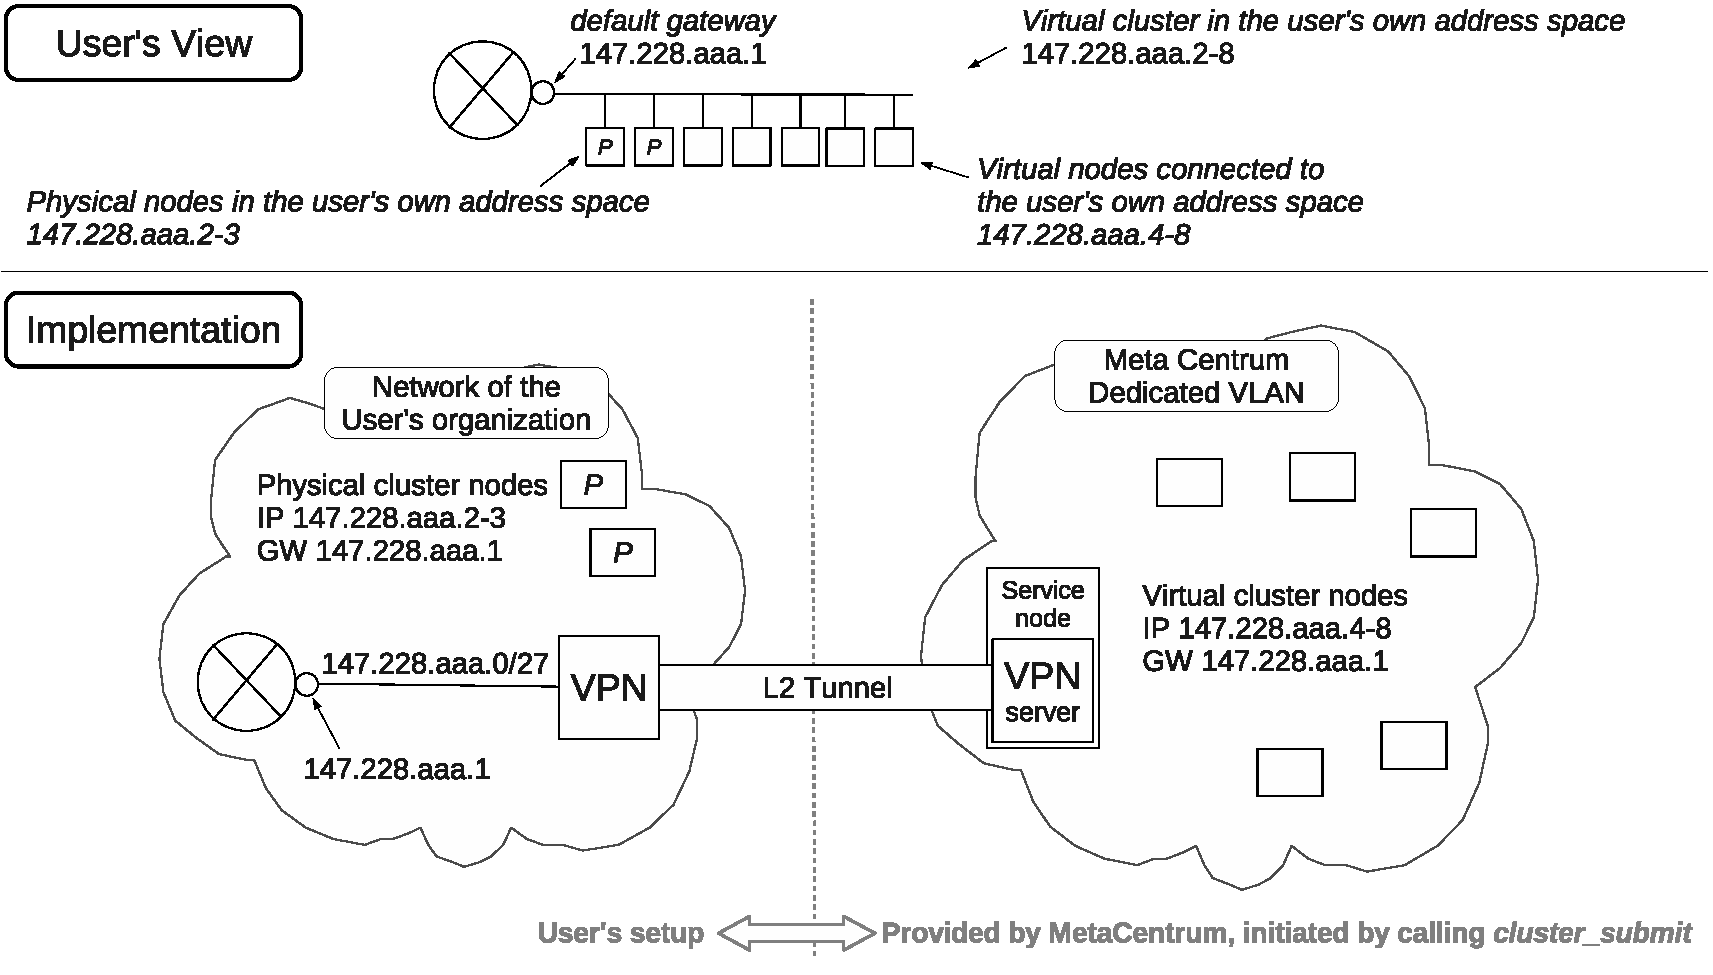
\includegraphics[width=\columnwidth]{publ.pdf}
    \caption{Virtual cluster publication as a part of user network}
    \label{fig:publication}
\end{figure}

Figure~\ref{fig:publication} shows the situation. There are two views
of the same reality. User view of the cluster
is ``just the departmental cluster,'' only that hardware resources have
been added (physically hosted in MetaCentrum).

From implementation point of view, we first describe the right half,
provided by MetaCentrum on user request to create new private virtual cluster. 
The virtual cluster consists of several virtual machines and one VLAN realized by  
advanced CESNET core network services (VPLS/Xponder
based, see \cite{virtcloud-techrep} for details).
The VLAN is completely isolated at the MetaCentrum level and
the only connection to the outside network is realized on the service
machine by means of tunneling to user's home network. The server side of the 
tunnel is implemented by an OpenVPN server running at the
service node of the virtual
cluster. That node is set up automatically by the virtual cluster management
services. 

The user side of the tunnel is implemented by an OpenVPN client
configured by the user as described below. For the
user part, see the left half of the implementation on
Fig.~\ref{fig:publication}. The user provides his/her end of the tunnel and
routing for the virtual cluster nodes in exactly the same way as he/she
provides for the physical local nodes (referenced as P in the figure).

OpenVPN is nevertheless intended to connect a single interface to a distant
(``corporate'') LAN. The modus operandi is slightly different here: we
connect a distant cluster to a LAN. The OpenVPN client is not ready to
attach a network to a remote LAN, just an interface.
This can be solved by Ethernet bridging
not only on the service machine side, but also at the client side.

The OpenVPN client configuration is the following:
\begin{verbatim}
dev tap
proto tcp-client
port 8080
remote 147.251.11.111
ping 1
ping-restart 45
ping-timer-rem
persist-tun
persist-key
verb 3
cert /etc/openvpn/mp_cert.pem
key /etc/openvpn/mp_key.pem
ca /etc/openvpn/ca.pem
tls-client
\end{verbatim}
where \verb'ca.pem' is the CESNET certificate, \verb'mp_cert.pem' and
\verb'mp_key.pem' are the user certificate and key. The user starts OpenVPN
with this configuration.

If the OpenVPN shall connect the cluster network with the user's home
network, following steps are necessary to provide appropriate bridging:
\begin{verbatim}
brctl addbr br0
brctl addif br0 tap0
brctl addif br0 ethX
ifconfig br0 $ip netmask $mask up
ifconfig ethX 0.0.0.0 up
ifconfig tap0 up
\end{verbatim}
where \verb'ethX' is an interface in the network to be connected,
\verb'$ip' is an address in that network, and \verb'$mask' is its mask.

If the machine is multihomed, it is also necessary to remove the default
route.

\subsubsection{MetaCenter Services Access Shortcuts}

The configuration described above is sufficient from functional point of
view; the virtual cluster is able to reach all the MetaCenter services in
such a configuration. It may be inadequate in performance, as all the
network traffic from the virtual cluster (physically set in the MetaCenter)
traverses user's home network also in cases when internal MetaCenter
services are used, e.g., Kerberos and/or filesystem access.

Network Address Translation (NAT) can be used to provide such a shortcut.
Using NAT has several advantages.
The machines inside the virtual cluster access the services the same way as
if they are anywhere in the Internet, i.e., using the same addresses and/or
domain name. As
NAT is commonly used to ``enlarge'' the available address
space (breaking unfortunately the original end-to-end paradigms of the
Internet), most protocols are able to deal with that.

The service machine supports three networking scenarios related to NAT. First,
NAT is disabled and is up to user to set up proper networking either static or
dynamic using DHCP. Second, NAT is enabled without any exception, i.e., any
node of the virtual cluster can access outer network through the service
machine. Third, NAT is enabled but limited only to selected services and
servers in MetaCenter. Currently, the limited NAT allows access to AFS
and NFS servers and to all KDC (Kerberos) servers. Users can choose either
disabled or MetaCenter limited NAT. The least restrictive unlimited NAT is
reserved for use with MetaCenter-provided images, as it is practically
equivalent to publishing the cluster under MetaCenter address space.

When NAT is enabled, routing to MetaCenter servers outside the virtual
cluster must be set on all computation nodes in the cluster. In that case,
the DHCP server pushes static routes (default route for unlimited NAT and
set of routes just to the servers for limited NAT) to the nodes.

\subsubsection{NFS over NAT Performance}

NAT increases latency of network. NFS is highly sensitive to network latency
thus we provide basic evaluation of NFS behavior over NAT compared with standard
local network. We used set of tasks that suffer from network latency,
i.e., it uses many synchronous operations in the NFS protocol such as creating
files.

We evaluated NFS behavior using three operations: unpacking Linux
kernel sources (the \emph{untar} line), building the kernel (the \emph{make}
line), deleting built tree (the \emph{rm -rf} line). The last line shows round
trip time through NAT and through real network. The results can be found in 
Table~\ref{tab:nateval}. The measurements are wall clock times of the
operations, averages of five runs and appropriate measurement errors.
As we can see, the slowdown is significant. The slowdown corresponds to our
experiences of NFS performance relationship to link latency (also shown in
the table). The performance loss is also proportional to the number of
synchronous operations (mainly file creation). This is especially
significant in building the kernel that transfers files from storage to the
computation node and creates enormous amount of temporary files.
Determining the exact cause in the NAT transfer
as well as finding a reasonable solution for
traversing NFS traffic to the user cluster nevertheless
needs further investigation which is planned as future work.

\begin{table}[htb]
\begin{center}
\begin{tabular}{|l|c|c|}
\hline
\bf Operation & \bf Native NFS & \bf NFS over NAT \\
\hline
\hline
%untar & $83.27\pm3.74$s & $134.31\pm9.57$s \\
untar & $\hphantom{1}83\pm4$ s & $134\pm10$ s \\
\hline
%make & $183.30\pm6.18$s & $829.91\pm14.59$s \\
make & $183\pm7$ s & $830\pm15$ s \\
\hline
%rm -rf & $20.28\pm1.24$s & \hphantom{1}$48.10\pm5.77$s \\
rm -rf & $\hphantom{1}20 \pm1$ s & \hphantom{1}$48 \pm~6$ s \\
\hline
ping & 0.146 ms & 0.304 ms \\
\hline
\end{tabular}
\end{center}
\caption{Performance limitations of NFS over NAT}
\label{tab:nateval}
\end{table}

\section{Authorization}
\label{Authorization}

Various security related issues had to be addressed during implementation of virtual clusters. Problems related to 
non-trusted node images and their encapsulation in private network were discussed in Section~\ref{sec:net}. 
In this section, authorization related development is described. 

\subsection{Architecture}
We use a common authorization framework designed and implemented in
MetaCentrum context \cite{metaauth}. It is based on groups and roles
or privileges associated to this groups. 


\begin{figure}[htb]
\begin{center}
    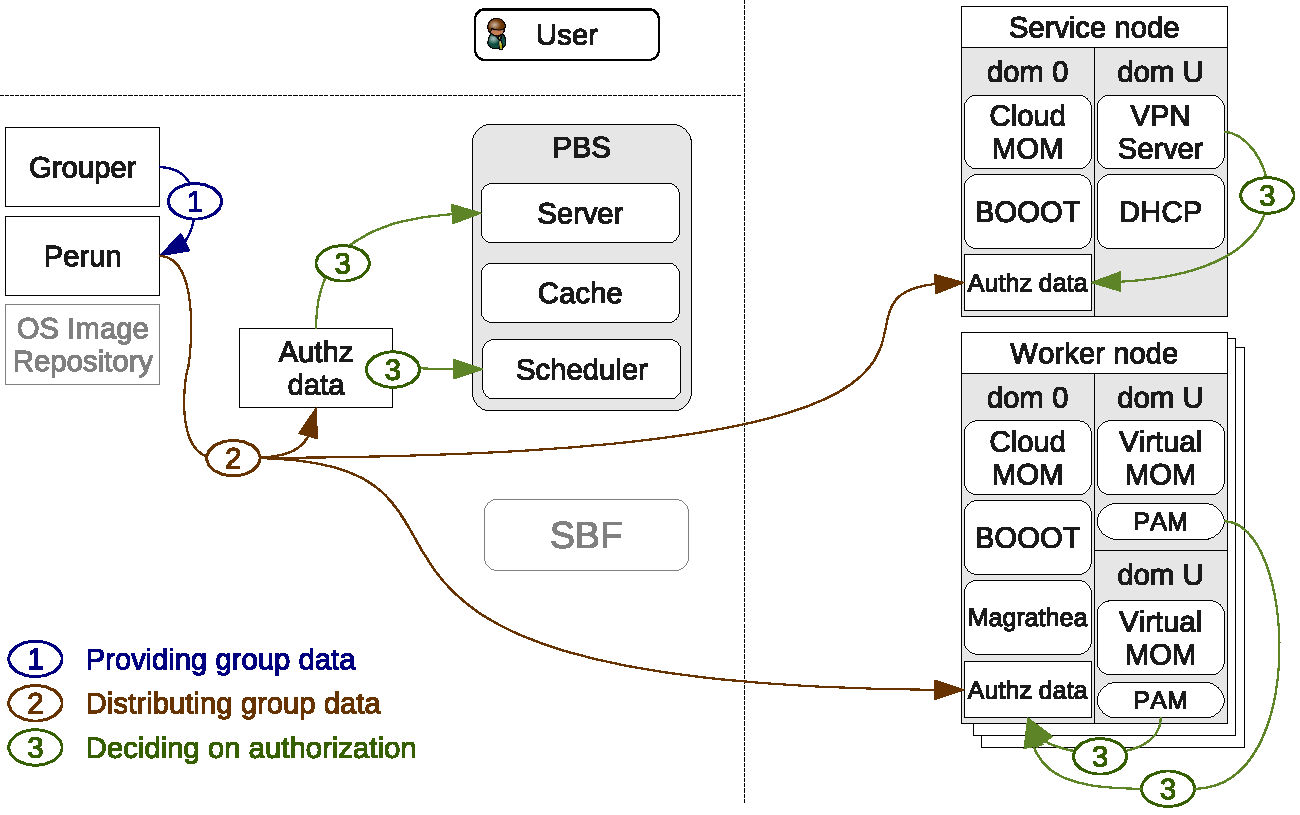
\includegraphics[width=.8\columnwidth]{auth_arch.pdf}
\end{center}
    \caption{Overall architecture of the virtual clouds solution}
    \label{fig:authz}
\end{figure}

The architecture consists of three parts (see Fig.~\ref{fig:authz}):
\begin{description}
 \item [group management]---definition of groups and its membership
   is a common task provided for all the MetaCentrum services by a
   single service based on Grouper~\cite{grouper}
 \item [authorization data distribution]---the MetaCentrum management
   tool, Perun~\cite{Perun}, is responsible for distributing the
   group membership information to the services. The Perun service
   provides all nodes with a up-to-date copy of group membership
   information in the form of a local file
 \item [decision points]---services uses the authorization
   information to make the decision. It is responsibility of each service
   to assign particular privileges to groups
\end{description}

\subsection{Decision points}
Authorization decisions should be done on several services:
\begin{description}
\item[cluster management]---cluster management rights are associated with
container job, representing the whole cluster. 
By default, only the container owner can manipulate with the cluster (e.g.,
to shutdown it). Cluster specification 
command supports parameter defining group of users with cluster management privileges. Both standard unix group and group 
defined by Grouper tool (\cite{grouper}) are supported on the PBS Server. Implementation is straightforward for users, 
group mechanism is already supported by PBSPro for limiting access to privileged queues. Our implementation follows the same strategy, 
with additional support for MetaCentrum authorization service~\cite{metaauth}. 
\item[job submit into cluster]---the same group authorization mechanism is
implemented in the PBS Scheduler, for decision 
whether user can submit jobs into cluster managed by the central PBSPro. In future work, groups defining access to cluster and management of
cluster could be split.
\item[access right on VPN server]---the service machine authorize the users
according to their certificates, in particular their DN from the certificates.
The DNs are maintained in a file on the service machine, this file is updated
by a Perun service.
\item[access to private worker nodes]---nodes installed from user-supplied images are completely under user control. MetaCentrum 
administrators don't have root access to these nodes and it is up to image owners to implement their own authorization. Several 
techniques are suggested, started from pre-allowed ssh access based on
private keys, to Kerberos based access control using MetaCentrum
Kerberos realm.
\item[access to public worker nodes]---access to publicly available
computation nodes is currently not limited, analogically to access to
standard computation nodes. MetaCentrum installation of nodes contains cleaning processes, which are responsible for monitoring user activities
and disallowing longer processes of users not running jobs on cluster
nodes. In near future, a new Linux PAM based module is planned, which
may deny access of those users to such nodes completely.

\item[privileges on Magrathea]---authorization decisions could be done also on Magrathea service, providing to cluster owners possibility 
to restart complete virtual machine belonging to the cluster. Such a
functionality is planned to be implemented next year.
\end{description}

\section{Related Work}

As virtualisation has recently become very popular in high performance
computing, several projects have emerged to deal with virtual machines
on worker nodes of computational clusters. As for the original motivation,
probably the closest project to ours is~\cite{karlsruhe}. Another interesting project aims to provide dynamic virtual
clustering~\cite{dvc} (DVC) using Xen virtual machine monitor, Moab workload
manager and Torque resource manager. Working in cooperation with Moab
developers the authors of DVC managed to provide transparent creation of
clusters of virtual machines. Virtual clusters are also allowed to span
multiple physical clusters by borrowing required resources from resource
managers of those clusters. Integration of virtual machines to batch systems 
in EGEE project was motivation for work in \cite{irove}. Similar development 
was done in~\cite{cern}, where virtual machines are integrated with PANDA framework, using LSF batch system.

The idea of complete clusters of virtual machines, built on-demand and according to user specification, is 
one of the key features of clouds \cite{amazon}. Two open-source implementations of cloud technology \cite{workspaces,eucalyptus} 
can be referred as examples of cloud infrastructure, which allows user-supplied images of nodes to be started on
remote resources and arranged to sets of nodes comprising one group.

Management of virtual images was studied in \cite{appliances}, where a virtual appliance, as an application 
combined with an environment required by the application, was defined. Management and deployment of such images was 
studied for example in \cite{teragrid2007}, which also motivated our work. Several pre-installed images 
(including OSG and CernVM images) can be found in repository on \url{http://workspace.globus.org/vm/marketplace.html}.

A representative list of work related to the networking scheme has been
given in our work~\cite{virtcloud-techrep}.

Our work contributes to the world-wide effort by introducing characteristic cloud features into the HPC environment, and making them accessible---with minimal modifications---through traditional batch system interfaces. Integration with advanced networking services constitutes a complete solution for encapsulating virtual computing resources in virtual networks. Integration with cloud interfaces (Globus Workspaces) is going to continue in the future.

\section{Conclusion}

A prototype has already been deployed and the development has been catering for the needs of early adopters.
In foreseeable future, the solution will be made available across the whole National Grid Infrastructure and the development team will focus its efforts on its further evolution.

In the short term, the service will be extended with other features such as group authorization mechanisms, allowing owners to delegate permissions to handle (turn off, restart) their virtual clusters. Also, a virtual image repository service will be designed to handle standard images as well as custom images submitted by users.

Long-term goals include integration with cloud interfaces and extension of the system to support not only PBSPro but other batch job systems such as Torque as well.

\subsection*{Acknowledgments} 
%\begin{acknowledgement}
This work was done with the support of Ministry of Education of the Czech
Republic, research programs MSM0021622419 and MSM6383917201.
%\end{acknowledgement}

	\begin{thebibliography}{10}
	\bibitem{sc07} Ruda, M.; Denemark, J.; Matyska, L.: \emph{Scheduling Virtual Grids: the Magrathea System},
	   Second International Workshop on Virtualization Technology in Distributed Computing, USA,
	   ACM digital library, 2007. p. 1-7. 2007, Reno, USA.
	\bibitem{sbf}Anto\v s, D.; Matyska, L.; Holub, P.; Sitera, J.: \emph{VirtCloud: Virtualising Network
	   for Grid Environments-First Experiences}, The 23rd IEEE International Conference on Advanced
	   Information Networking and Applications AINA 2009. Bradford, UK : IEEE Comp. Soc., 2009. pp.
	   876-883, 8 p. ISBN 978-0-7695-3638-5
        \bibitem{VirtCloud-CGW08}
         Anto\v s, D., Sitera, J., Matyska, L., Holub, P.: \emph{MetaCenter
         Virtual Networks}. In Cracow Grid Workshop 2008. Cracow, Poland : Cyfronet
         AGH, Krak\'ow, Poland, 2009. pp. 86-93, 8 p. ISBN 9788361433002.
	\bibitem{karlsruhe}
	V. B\"uge, Y. Kemp, M. Kunze, O. Oberst, and G. Quast.
	\emph{Virtualizing a Batch Queuing System at a University Grid Center.}
	In {Frontiers of High Performance Computing and Networking---ISPA
	Workshops}, Springer-Verlag LNCS 4331, 2006.
	\bibitem{dvc}
	W. Emeneker, D. Jackson, K. Butikofer, D. Stanzione.
	\emph{Dynamic Virtual Clustering with Xen and Moab}.
	In {Frontiers of High Performance Computing and Networking---ISPA
	Workshops}, Springer-Verlag LNCS 4331, 2006.
	\bibitem{workspaces}
	K. Keahey, K. Doering, and I. Foster. From Sandbox to Playground: \emph{Dynamic Virtual
	Environments in the Grid.} In: {5th International Workshop in Grid Computing
	(Grid 2004)}. 2004.
	\bibitem{cern}
	O. Khalid; Richard J. Anthony; P. Nilsson; K. Keahey; M. Schulz; K. Parrot; M. Petridis:
	\emph{Enabling and optimizing pilot jobs using xen based virtual machines for the HPC grid applications.} In
	VTDC '09: Workshop on Virtualization technologies in distributed computing,
	2009, Barcelona, Spain.
	\bibitem{irove}
	S. Childs, B. Coghlan, and J. McCandless. \emph{Dynamic virtual worker nodes in a production Grid.} 
        In Frontiers of High Performance Computing and Networking - ISPA
	2006 Workshops (XHPC 2006), volume 4331/2006, pages 417-426, Sorrento, Italy, December 2006.
	\bibitem{eucalyptus} Nurmi D., Wolski r., Grzegorczyk Ch., Obertelli G.,
	    Soman S., Youseff L., and Zagorodnov D. \emph{The eucalyptus
	    open-source cloud-computing system.} In Proceedings of Cloud
	    Computing and Its Applications, October 2008.
	\bibitem{teragrid2007}Bradshaw, R., N. Desai, T. Freeman, K. Keahey. 
        \emph{A Scalable Approach To Deploying And Managing Appliances.} TeraGrid 2007, Madison, WI. June
	2007.
	\bibitem{appliances} Sapuntzakis C., Brumley D., Chandra R., Zeldovich N., Chow J., Lam M. S., and Rosenblum M..
	\emph{Virtual Appliances for Deploying and Maintaining Software.}
	In Proceedings of the Seventeenth Large Installation Systems Administration Conference (LISA 2003), San Diego, CA, pages 181-194, October 2003.
	\bibitem{amazon}Amazon Web Services. Amazon Elastic Compute Cloud (ec2). \url{http://aws.amazon.com/ec2}
        \bibitem{virtcloud-techrep} D. Anto\v s, L. Matyska, P. Holub, and J.
        Sitera.
        \emph{VirtCloud: Virtual Network for User-controlled Virtual
        Clusters}. CESNET Technical Report 1/2009. 2009.
        \bibitem{Perun} K\v renek A., Sebestianov\'a Z. \emph{Perun -- 
        Fault-Tolerant Management of Grid Resources}, Cracow Grid
        Workshop'04 Proceedings, Academic Computer Centre CYFRONET
        AGH, 2005, pages 133-140, ISBN: 83-915141-4-5
\bibitem{grouper}Grouper, project home page. 
\url{http://grouper.internet2.edu/}. 2009.
\bibitem{metaauth} Daniel Kouril, Michal Prochazka.
Fault-tolerant Access Control in Distributed Environment
- the MetaCentrum Authorization Infrastructure.
CESNET Technical Report XX/2009, submitted on Dec 5th, 2009. To appear.
\bibitem{xen}
P. Barham, B. Dragovic, K. Fraser, S.
Hand, T. Harris, A. Ho, R. Neugebar, I. Pratt, and A.
Warfield. Xen and the Art of Virtualization. In {\em ACM
Symposium on Operating Systems Principles (SOSP)}. October 2003.
\bibitem{vserver}
Stephen Soltesz, Herbert Potzl, Marc E. Fiuczynski, Andy Bavier and Larry Peterson.
Container-based
Operating System Virtualization: A Scalable, High-performance Alternative to
Hypervisors. April 2007.
	\end{thebibliography}

\end{document} 
